% ===================================================================
%  Week 13 — Persian lecture notes — Convolutional Neural Networks
% ===================================================================
\documentclass[12pt,a4paper]{article}
% ===================================================================
%  Shared preamble for Persian lecture notes (Image Processing).
%  Compile with XeLaTeX.  Body = Persian (RTL), code/math = LTR.
% ===================================================================

\usepackage{geometry}
\geometry{a4paper,margin=2.4cm}
\usepackage{amsmath,amssymb}
\usepackage{graphicx}
\usepackage{xcolor}
\usepackage{listings}
\usepackage{tcolorbox}
\usepackage{booktabs}
\usepackage{array}
\usepackage{enumitem}
\usepackage{hyperref}
\tcbuselibrary{skins,breakable}

% ---- Persian / RTL --------------------------------------------------
\usepackage{xepersian}
\settextfont{IRNazli}
\setlatintextfont{Latin Modern Roman}
\setdigitfont{IRNazli}
% More generous leading + paragraph spacing (Persian reads better with air).
\linespread{1.5}
\setlength{\parskip}{0.7em}

% ---- Colours --------------------------------------------------------
\definecolor{coursePrimary}{HTML}{1B4965}
\definecolor{courseAccent}{HTML}{E76F51}
\definecolor{courseGood}{HTML}{2A9D8F}
\definecolor{courseBad}{HTML}{C0392B}
\definecolor{courseInfo}{HTML}{2980B9}
\definecolor{codeBg}{HTML}{F5F6FA}
\definecolor{codeKw}{HTML}{8E44AD}
\definecolor{codeStr}{HTML}{2A9D8F}
\definecolor{codeCom}{HTML}{7F8C8D}

\hypersetup{colorlinks=true,linkcolor=courseInfo,urlcolor=courseInfo,citecolor=courseInfo}

% ---- Code listings (Python built in) -------------------------------
\lstdefinestyle{course}{
  backgroundcolor=\color{codeBg},
  basicstyle=\ttfamily\small,
  keywordstyle=\color{codeKw}\bfseries,
  stringstyle=\color{codeStr},
  commentstyle=\color{codeCom}\itshape,
  numberstyle=\tiny\color{codeCom},
  numbers=left, numbersep=7pt,
  showstringspaces=false, breaklines=true,
  tabsize=4, columns=fullflexible, frame=single,
  rulecolor=\color{gray!30}, keepspaces=true, upquote=true, language=Python,
}
\lstset{style=course}
\lstdefinelanguage{bash}{
  keywords={cd,pip,python,venv,source,import}, sensitive=true,
  morecomment=[l]{\#}, morestring=[b]', morestring=[b]",
}
\newenvironment{ltrcode}{\begin{LTR}}{\end{LTR}}

% ---- Callout boxes (Persian titles) --------------------------------
\newtcolorbox{yaddasht}{colback=courseInfo!8,colframe=courseInfo,
  title={\textbf{یادداشت}},boxrule=0.6pt,right=6pt,left=6pt,breakable}
\newtcolorbox{nokte}{colback=courseAccent!10,colframe=courseAccent,
  title={\textbf{نکتهٔ کلیدی}},boxrule=0.6pt,right=6pt,left=6pt,breakable}
\newtcolorbox{hoshdar}{colback=courseBad!8,colframe=courseBad,
  title={\textbf{هشدار / دام}},boxrule=0.6pt,right=6pt,left=6pt,breakable}
\newtcolorbox{riyazi}{colback=coursePrimary!6,colframe=coursePrimary,
  title={\textbf{ریاضیات}},boxrule=0.6pt,right=6pt,left=6pt,breakable}
\newtcolorbox{tamrin}{colback=courseGood!8,colframe=courseGood,
  title={\textbf{تمرین}},boxrule=0.6pt,right=6pt,left=6pt,breakable}

% ---- Header helper --------------------------------------------------
\newcommand{\coursemeta}[2]{%
  \begin{center}
  {\large\textbf{پردازش تصویرِ کاربردی}}\\[2pt]
  {\color{coursePrimary}\rule{\linewidth}{1pt}}\\[4pt]
  {\Large\textbf{#1}}\\[3pt]
  {\small جزوهٔ درس — #2}
  \end{center}\vspace{4pt}
}


\begin{document}
\coursemeta{جلسهٔ ۱۳ — شبکه‌های عصبیِ کانولوشنی (Convolutional Neural Networks)}{هفتهٔ سیزدهم}

\section*{نگاهِ کلی به این جلسه}

این جلسه اوجِ بخشِ یادگیریِ درس است. در هفتهٔ ۳، \emph{ما} کرنل‌ها را با دست طراحی کردیم (بلور، سوبل) و اعدادشان را خودمان انتخاب کردیم. در هفتهٔ ۱۲ دیدیم که ویژگی‌های دست‌طراحی (HOG) به سقف می‌خورند. امروز ایدهٔ بزرگ را می‌آموزیم: بگذاریم شبکه \textbf{خودِ کرنل‌ها را از داده یاد بگیرد} — و هم‌زمان طبقه‌بند را هم یاد بگیرد. این همان \textbf{شبکهٔ عصبیِ کانولوشنی} (CNN) است، ستون‌فقراتِ بینایی ماشینِ مدرن.

\begin{yaddasht}
نتیجهٔ واقعیِ امروز: یک CNNِ کوچک، ارقامِ ۰ تا ۹ را با دقتِ \textbf{۹۷٪} می‌خواند. این دقیقاً همان «خوانندهٔ ارقامِ کنتور» است که DocScan به آن نیاز دارد — و آن را از صفر آموزش می‌دهیم. جالب اینکه روی همین ارقامِ ساده، یک SVMِ کلاسیک هم ۹۹٪ می‌گیرد؛ این تضاد، درسِ صادقانه‌ای دربارهٔ «کِی CNN واقعاً برنده است» به ما می‌دهد.
\end{yaddasht}

\subsection*{یک تشبیهِ ساده}

تصور کنید یک کارآموزِ کنترلِ کیفیت می‌خواهد قطعاتِ سالم را از معیوب تشخیص دهد. در روشِ کلاسیک، سرپرست به او فهرستی از قواعد می‌دهد: «این خراش را ببین، آن لبه را چک کن». در روشِ CNN، به کارآموز هزاران قطعهٔ برچسب‌دار نشان می‌دهند و او \emph{خودش} کم‌کم یاد می‌گیرد به چه نشانه‌هایی نگاه کند — و این نشانه‌ها را کسی از پیش به او نگفته. جالب‌تر اینکه او ابتدا نشانه‌های ساده (لبه، رنگ) را یاد می‌گیرد و بعد آن‌ها را در قالبِ الگوهای پیچیده‌تر ترکیب می‌کند. CNN دقیقاً همین‌گونه است: سلسله‌ای از لایه‌ها که هر کدام الگوی پیچیده‌تری از لایهٔ قبل می‌سازد، و همهٔ این «یادگرفتنِ نشانه‌ها» از دادهٔ برچسب‌دار می‌آید.

\section{از کرنل تا فیلترِ آموخته‌شده}

\subsection{کانولوشن: شما از قبل بلدید}

در هفتهٔ ۳ یاد گرفتیم: یک کرنلِ کوچک را روی تصویر می‌لغزانیم، ضرب‌ودرجمع می‌کنیم و یک تصویرِ فیلترشده می‌گیریم. کرنلِ سوبل لبه‌ها را پیدا می‌کند و کرنلِ بلور صاف می‌کند. \emph{ما} اعداد را انتخاب می‌کردیم.

یک \textbf{لایهٔ کانولوشنی} دقیقاً همین عملیات است — با این تفاوتِ حیاتی که اعدادِ کرنل \textbf{آموخته} می‌شوند، نه دستی انتخاب.

\begin{nokte}
ساده‌ترین تعریفِ CNN: «کانولوشن با کرنل‌هایی که با آموزش انتخاب می‌شوند، نه با دست». همهٔ پیچیدگیِ ظاهری از همین ایدهٔ ساده می‌آید.
\end{nokte}

\subsection{شبکه چه چیزی یاد می‌گیرد؟}

پس از آموزشِ CNNِ ارقامِ ما، هشت فیلترِ $۳\times۳$ لایهٔ اول را که شبکه \emph{یاد گرفته} استخراج کردیم:

\begin{center}
  
\includegraphics[width=0.7\linewidth]{../assets/learned_filters.png}\\
  {\small ۸ فیلترِ لایهٔ اول که CNN برای خواندنِ ارقام یاد گرفت — هیچ‌کس آن‌ها را طراحی نکرد}
\end{center}

هیچ‌کس این اعداد را انتخاب نکرد؛ گرادیان کاهشی (gradient descent) آشکارسازهای لبه/خطِ مفید برای تشخیصِ ارقام را پیدا کرد. لایه‌های اولیه لبه‌ها را یاد می‌گیرند، لایه‌های عمیق‌تر آن‌ها را در قالبِ اجزا و سپس شکل‌های کامل ترکیب می‌کنند.

\subsection{یک مثالِ عددیِ کانولوشن (یادآوریِ هفتهٔ ۳)}

بیایید مطمئن شویم کانولوشن را دقیق به یاد داریم. فرض کنید یک تکه از تصویر و یک کرنلِ $۳\times۳$ داریم:

\begin{riyazi}
\[
\text{تکهٔ تصویر}=\begin{pmatrix} 2 & 0 & 1 \\ 4 & 6 & 3 \\ 1 & 2 & 5 \end{pmatrix},\qquad
\text{کرنلِ لبهٔ عمودی}=\begin{pmatrix} -1 & 0 & 1 \\ -1 & 0 & 1 \\ -1 & 0 & 1 \end{pmatrix}
\]
خروجیِ کانولوشن در مرکز = مجموعِ ضربِ عنصر‌به‌عنصر:
\[
(2)(-1)+(0)(0)+(1)(1) + (4)(-1)+(6)(0)+(3)(1) + (1)(-1)+(2)(0)+(5)(1)
\]
\[
= (-2+0+1) + (-4+0+3) + (-1+0+5) = -1 -1 +4 = 2
\]
\end{riyazi}

این عددِ $۲$ می‌گوید «در این نقطه یک لبهٔ عمودیِ ملایم (روشن‌تر در سمتِ راست) وجود دارد». در هفتهٔ ۳ ما این کرنلِ $[-1,0,1]$ را \emph{انتخاب} کردیم. در CNN، شبکه با آموزش کشف می‌کند که چنین کرنلی مفید است و اعدادش را خودش تنظیم می‌کند. تفاوت فقط در «چه کسی اعداد را انتخاب می‌کند» است.

\begin{nokte}
این پیوند حیاتی است: CNN چیزِ کاملاً جدیدی اختراع نکرده؛ همان کانولوشنِ آشنا را گرفته و فقط انتخابِ کرنل را از انسان به الگوریتمِ آموزش سپرده است.
\end{nokte}

\subsection{نقشهٔ ویژگی}

اعمالِ یک فیلترِ آموخته‌شده روی تصویر، یک \textbf{نقشهٔ ویژگی} (feature map) می‌دهد: نقشه‌ای که نشان می‌دهد آن الگو کجای تصویر ظاهر شده. یک لایه چندین فیلتر دارد، پس چندین نقشهٔ ویژگی تولید می‌کند — یک «پشته» از آشکارسازهای الگو. لایهٔ بعدی روی این پشته کانولوشن می‌زند و الگوهای ساده را به الگوهای پیچیده تبدیل می‌کند.

\section{کالبدشکافیِ یک CNN}

یک CNN از چند نوع لایه ساخته می‌شود:

\begin{center}
\begin{tabular}{@{}lll@{}}
\hline
\textbf{لایه} & \textbf{کارش} & \textbf{چرا} \\
\hline
کانولوشن & فیلترهای آموخته $\rightarrow$ نقشه‌های ویژگی & کشفِ الگو \\
ReLU & $\max(0,x)$ روی هر عنصر & افزودنِ غیرخطی‌بودن \\
Pooling & کوچک‌سازی (مثلاً بیشینهٔ $۲\times۲$) & کوچک‌سازی + ناوردایی \\
تمام‌متصل (FC) & تخت‌کردن $\rightarrow$ امتیازِ کلاس‌ها & تصمیمِ نهایی \\
Softmax & امتیاز $\rightarrow$ احتمال & انتخابِ کلاس \\
\hline
\end{tabular}
\end{center}

\subsection{شمردنِ پارامترها}

بیایید بشماریم شبکهٔ کوچکِ ما چند پارامتر دارد — این عادتِ خوبی برای فهمِ اندازهٔ مدل است:

\begin{riyazi}
\begin{itemize}
  \item لایهٔ c1: ۸ فیلترِ $۳\times۳$ روی ۱ کانالِ ورودی $= 8\times(3\times3\times1) + 8\ \text{بایاس} = 80$ پارامتر.
  \item لایهٔ c2: ۱۶ فیلترِ $۳\times۳$ روی ۸ کانال $= 16\times(3\times3\times8) + 16 = 1168$ پارامتر.
  \item لایهٔ fc: از ۶۴ ورودی به ۱۰ خروجی $= 64\times10 + 10 = 650$ پارامتر.
  \item \textbf{مجموع} $\approx 1898$ پارامتر.
\end{itemize}
\end{riyazi}

\begin{nokte}
کمتر از ۲۰۰۰ پارامتر — بسیار کوچک! برای مقایسه، AlexNet حدودِ ۶۰ میلیون و ResNet-۵۰ حدودِ ۲۵ میلیون پارامتر دارد. همین شبکهٔ ریز، ارقام را با ۹۷٪ می‌خواند، چون مسئله ساده است و معماریِ کانولوشنی برای تصویر بسیار کارآمد است.
\end{nokte}

\subsection{چرا ReLU (غیرخطی‌بودن)؟}

اگر فقط کانولوشن‌ها را روی هم بگذاریم، حاصل هنوز یک فیلترِ خطیِ بزرگ است — هیچ قدرتِ اضافه‌ای نمی‌گیریم.

\begin{riyazi}
ترکیبِ عملیاتِ خطی باز هم خطی است: اگر $f(x)=Ax$ و $g(x)=Bx$، آن‌گاه $g(f(x))=BAx$ که باز هم یک تبدیلِ خطیِ واحد است. برای رهایی از این دام، بینِ لایه‌ها یک تابعِ \emph{غیرخطی} می‌گذاریم. \textbf{ReLU} یعنی $\mathrm{ReLU}(x)=\max(0,x)$: هر مقدارِ منفی را صفر می‌کند و مثبت‌ها را دست‌نخورده می‌گذارد.
\end{riyazi}

\begin{nokte}
بدونِ غیرخطی‌بودن، ده لایهٔ کانولوشن به یک لایه فرومی‌کاهند. ReLU همان چیزی است که واژهٔ «عمیق» را معنادار می‌کند.
\end{nokte}

\subsection{چرا Pooling؟}

\textbf{بیشینه‌گیری} (max-pooling) در هر پنجرهٔ کوچک، قوی‌ترین پاسخ را نگه می‌دارد و اندازه را نصف می‌کند. سه فایده:

\begin{itemize}
  \item \textbf{تحملِ جابه‌جایی:} رقمی که یک پیکسل جابه‌جا شده، باز همان واحدها را فعال می‌کند.
  \item \textbf{کاهشِ محاسبات:} تصویرِ کوچک‌تر یعنی پردازشِ سریع‌تر.
  \item \textbf{رشدِ میدانِ دید:} لایه‌های بعدی ناحیهٔ بزرگ‌تری از تصویرِ اصلی را «می‌بینند».
\end{itemize}

\begin{yaddasht}
شهودِ pooling: «این الگو را جایی در این ناحیه دیدم»، نه «دقیقاً در این پیکسل». همین کمی ابهامِ مکانی، شبکه را در برابرِ جابه‌جاییِ کوچک مقاوم می‌کند.
\end{yaddasht}

\subsection{Softmax با یک مثالِ عددی}

لایهٔ آخر ۱۰ عددِ خام (logit) می‌دهد که می‌توانند هر مقداری باشند. \textbf{Softmax} آن‌ها را به احتمال‌هایی تبدیل می‌کند که جمعشان ۱ می‌شود.

\begin{riyazi}
برای امتیازهای خام $z$، احتمالِ کلاسِ $i$:
\[
p_i = \frac{e^{z_i}}{\sum_j e^{z_j}}
\]
مثال: اگر سه امتیازِ خام $z=[2.0,\ 1.0,\ 0.1]$ باشند:
\[
e^{2.0}=7.39,\quad e^{1.0}=2.72,\quad e^{0.1}=1.11,\quad \text{مجموع}=11.22
\]
\[
p = [0.66,\ 0.24,\ 0.10]
\]
پس شبکه با احتمالِ ۶۶٪ کلاسِ اول را پیش‌بینی می‌کند. توجه کنید که softmax اختلاف‌ها را تشدید می‌کند (نمایی است) و همیشه خروجیِ مثبت با جمعِ ۱ می‌دهد.
\end{riyazi}

\begin{nokte}
چرا نمایی؟ چون هم همه‌چیز را مثبت می‌کند و هم به امتیازهای بزرگ‌تر وزنِ به‌مراتب بیشتری می‌دهد — که رفتارِ «انتخابِ برنده» را مدل می‌کند. سپس آنتروپیِ متقاطع روی همین احتمال‌ها زیان را حساب می‌کند.
\end{nokte}

\subsection{CNNِ ارقامِ ما، سرتاسر}

\begin{itemize}
  \item ورودی: رقمِ $۸\times۸$ $\rightarrow$ کانولوشن (۸ فیلتر)+ReLU+Pool $\rightarrow$ $۴\times۴$.
  \item $\rightarrow$ کانولوشن (۱۶ فیلتر)+ReLU+Pool $\rightarrow$ $۲\times۲$ $\rightarrow$ تخت‌سازی (۶۴) $\rightarrow$ FC $\rightarrow$ ۱۰ امتیاز.
  \item Softmax ده امتیاز را به احتمال تبدیل می‌کند؛ بزرگ‌ترین احتمال، رقمِ پیش‌بینی‌شده است.
\end{itemize}

دو بلوکِ کانولوشن و یک لایهٔ خطی — با معیارهای امروزی بسیار کوچک، اما همین ارقام را با ۹۷٪ می‌خواند.

\section{آموزشِ یک CNN}

شبکه چطور فیلترها را یاد می‌گیرد؟ چهار گامِ تکرارشونده:

\begin{enumerate}
  \item \textbf{گذرِ رو‌به‌جلو (forward):} تصویر را از شبکه عبور بده و احتمال‌های پیش‌بینی‌شده را بگیر.
  \item \textbf{زیان (loss):} اندازه بگیر چقدر اشتباه است (آنتروپیِ متقاطع بینِ پیش‌بینی و برچسبِ واقعی).
  \item \textbf{پس‌انتشار (backprop):} حساب کن هر وزن چقدر در زیان اثر داشت (گرادیان).
  \item \textbf{به‌روزرسانی (update):} هر وزن را کمی در جهتِ کاهشِ زیان تغییر بده (گرادیان کاهشی).
\end{enumerate}

این چرخه روی هزاران تصویر و ده‌ها epoch تکرار می‌شود و فیلترها به‌تدریج به آشکارسازهای خوب تبدیل می‌شوند.

\subsection{زیانِ آنتروپیِ متقاطع}

\begin{riyazi}
شبکه برای هر کلاس یک احتمال می‌دهد. زیانِ آنتروپیِ متقاطع برای یک نمونه:
\[
L = -\log\big(p_{\text{کلاسِ درست}}\big)
\]
اگر شبکه به کلاسِ درست احتمالِ بالا بدهد، $p\to1$ و $L\to0$. اگر با اطمینان اشتباه کند ($p\to0$)، زیان به‌شدت بزرگ می‌شود. آموزش، میانگینِ این زیان را روی کلِ داده کمینه می‌کند.
\end{riyazi}

\subsection{گرادیان کاهشی، شهودی}

پس‌انتشار و گرادیان کاهشی قلبِ آموزش‌اند. شهودِ ساده: تصور کنید در مهی غلیظ روی یک تپه ایستاده‌اید و می‌خواهید به پایین‌ترین نقطهٔ دره برسید.

\begin{riyazi}
شما شیبِ زمین را زیرِ پایتان حس می‌کنید (این همان \emph{گرادیان} است) و یک گامِ کوچک در جهتِ سراشیبی برمی‌دارید. اندازهٔ گام همان \emph{نرخِ یادگیری} است. با تکرار، به کفِ دره (کمینهٔ زیان) نزدیک می‌شوید:
\[
w_{\text{جدید}} = w_{\text{قدیم}} - \eta \cdot \frac{\partial L}{\partial w}
\]
که $\eta$ نرخِ یادگیری و $\frac{\partial L}{\partial w}$ گرادیانِ زیان نسبت به وزن است. پس‌انتشار (backprop) روشی کارآمد برای محاسبهٔ این گرادیان برای \emph{همهٔ} وزن‌ها به‌طورِ هم‌زمان است.
\end{riyazi}

\begin{yaddasht}
گامِ خیلی بزرگ ($\eta$ بزرگ) ممکن است از روی دره بپرید و واگرا شوید؛ گامِ خیلی کوچک، رسیدن به کف را بی‌نهایت کند می‌کند. یافتنِ $\eta$ مناسب، مهم‌ترین تنظیمِ عملیِ آموزش است.
\end{yaddasht}

\subsection{آموزش در عمل}

منحنیِ آموزشِ واقعیِ CNNِ ما:

\begin{center}
  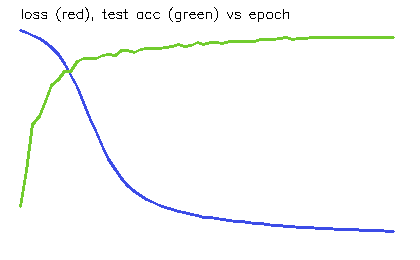
\includegraphics[width=0.6\linewidth]{../assets/training_curve.png}\\
  {\small قرمز: زیانِ آموزش (کاهشی) \quad سبز: دقتِ آزمون (صعودی تا نزدیکِ ۰٫۹۷)}
\end{center}

خطِ قرمز (زیان) هر epoch پایین می‌آید و خطِ سبز (دقتِ آزمون) بالا می‌رود و سپس به سقف می‌رسد. تماشای هم‌زمانِ این دو منحنی، راهِ زندهٔ تشخیصِ کم‌برازش/بیش‌برازش است.

\subsection{دسته‌های کوچک، epoch، نرخِ یادگیری}

\begin{itemize}
  \item \textbf{دستهٔ کوچک (mini-batch):} به‌جای کلِ داده، هر بار روی گروهی کوچک (ما ۱۲۸ تصویر) به‌روزرسانی می‌کنیم — سریع‌تر و نرم‌تر.
  \item \textbf{epoch:} یک گذرِ کامل روی کلِ دادهٔ آموزش. ما ۶۰ تا اجرا کردیم.
  \item \textbf{نرخِ یادگیری (learning rate):} اندازهٔ هر گامِ به‌روزرسانی. خیلی بزرگ $\rightarrow$ واگرایی؛ خیلی کوچک $\rightarrow$ کندیِ مفرط.
\end{itemize}

\begin{hoshdar}
بیشترِ شکست‌های آموزش از نرخِ یادگیریِ بد می‌آید. اگر زیان منفجر شد یا اصلاً حرکت نکرد، اولین چیزی که تغییر می‌دهید نرخِ یادگیری است.
\end{hoshdar}

\section{نتایج}

\subsection{خواندنِ ارقام — دستاوردِ DocScan}

\begin{center}
  
\includegraphics[width=0.75\linewidth]{../assets/predictions.png}\\
  {\small ارقامِ آزمون با پیش‌بینیِ CNN (سبز = درست). این همان خوانندهٔ ارقامِ کنتور است}
\end{center}

\subsection{CNN در برابرِ کلاسیک — مقایسهٔ صادقانه}

\begin{center}
\begin{tabular}{@{}lc@{}}
\hline
\textbf{روش} & \textbf{دقتِ آزمون (ارقام)} \\
\hline
CNN (فیلترهای آموخته) & ۰٫۹۷ \\
SVM روی پیکسلِ خام & ۰٫۹۹ \\
\hline
\end{tabular}
\end{center}

نکتهٔ صادقانه: روی ارقامِ \emph{ساده} و تمیزِ $۸\times۸$، یادگیریِ ماشینِ کلاسیک از قبل عالی است — CNN اینجا معجزه نمی‌کند. برتریِ واقعیِ CNN روی تصاویرِ \emph{سخت، بزرگ و متنوع} ظاهر می‌شود، و به‌ویژه با \textbf{یادگیریِ انتقالی} (هفتهٔ ۱۴).

\subsection{اشتراکِ وزن: چرا CNN از شبکهٔ کاملاً‌متصل بهتر است}

چرا اصلاً کانولوشن؟ چرا مثلِ شبکه‌های عصبیِ معمولی همهٔ پیکسل‌ها را به همهٔ نورون‌ها وصل نکنیم؟ دو دلیلِ قدرتمند:

\begin{riyazi}
\textbf{۱) اشتراکِ وزن (weight sharing):} یک کرنلِ $۳\times۳$ فقط ۹ وزن دارد که روی \emph{کلِ} تصویر لغزانده می‌شود. یک لایهٔ کاملاً‌متصل برای تصویرِ $۹۶\times۹۶$ به میلیون‌ها وزن نیاز دارد. کانولوشن با ۹ وزن همان کار را می‌کند — کارآمدیِ عظیم.

\textbf{۲) ناوردایی به مکان:} چون همان کرنل همه‌جا اعمال می‌شود، اگر یک رقم در گوشهٔ چپ یا راستِ تصویر باشد، با همان فیلتر شناسایی می‌شود. شبکهٔ کاملاً‌متصل باید این را جداگانه برای هر مکان یاد بگیرد.
\end{riyazi}

\begin{yaddasht}
این دو ویژگی — پارامترهای کم و ناوردایی به مکان — دلیلِ اصلیِ سلطهٔ CNN بر تصویر است. آن‌ها «سوگیریِ استقرایی» (inductive bias) مناسبِ داده‌های تصویری را در معماری تعبیه می‌کنند: می‌دانیم الگوهای مفید در تصویر محلی‌اند و می‌توانند هرجا ظاهر شوند.
\end{yaddasht}

\subsection{CNN کِی واقعاً برنده است؟}

\begin{itemize}
  \item مجموعه‌داده‌های بزرگ و متنوع که ویژگیِ دستی نمی‌تواند تنوعشان را بگیرد.
  \item مسائلی که ویژگیِ مفید در آن‌ها ناشناخته است (شبکه خودش کشفشان می‌کند).
  \item یادآوری هفتهٔ ۱۲: HOG+SVM روی خودروهای شبیه‌به‌هم روی ۴۸٪ متوقف شد — دقیقاً همان‌جا که ویژگیِ آموخته کمک می‌کند.
\end{itemize}

\begin{nokte}
قاعدهٔ سرانگشتی: مسئلهٔ کوچک و تمیز $\rightarrow$ کلاسیک کافی است. مسئلهٔ بزرگ و شلوغ $\rightarrow$ یادگیریِ عمیق جلو می‌افتد. یک مهندسِ خوب می‌داند کدام است.
\end{nokte}

\section{ژرف‌نگری}

\subsection{سلسله‌مراتبِ ویژگی}

\begin{itemize}
  \item لایهٔ ۱: لبه‌ها و خطوطِ ساده (مثلِ فیلترهای آموخته‌ای که دیدیم).
  \item لایهٔ ۲ و ۳: گوشه‌ها، منحنی‌ها، اجزای رقم (حلقه‌ها، محلِ اتصال).
  \item لایه‌های عمیق‌تر: آشکارسازهای شکلِ کامل که برای یک رقمِ خاص فعال می‌شوند.
\end{itemize}

CNN پیچیدگی را تدریجی می‌سازد: اجزای ساده در قالبِ کل‌های معنادار ترکیب می‌شوند، و همهٔ این‌ها آموخته می‌شوند.

\subsection{منظم‌سازی: صادق نگه‌داشتنِ CNN}

CNNها پارامترهای زیادی دارند، پس می‌توانند بیش‌برازش کنند (درسِ هفتهٔ ۱۲ بازمی‌گردد). ابزارهای مهار:

\begin{itemize}
  \item \textbf{Dropout:} در حینِ آموزش، به‌طورِ تصادفی برخی فعال‌سازی‌ها را صفر کن تا شبکه به هیچ واحدِ خاصی وابسته نشود.
  \item \textbf{افزایشِ داده (augmentation):} چرخش/جابه‌جاییِ تصادفیِ تصاویرِ آموزش — دادهٔ اضافیِ رایگان و ناورداییِ بیشتر.
  \item \textbf{کاهشِ وزن (weight decay):} جریمهٔ وزن‌های بزرگ برای سادّه‌نگه‌داشتنِ مدل.
\end{itemize}

\subsection{معماری‌های معروف: یک نگاهِ کوتاه}

CNNِ ما کوچک است، اما در دلِ همان خانواده‌ای است که تاریخِ بینایی ماشین را ساخت:

\begin{itemize}
  \item \textbf{LeNet-5} (۱۹۹۸، یان لوکون): اولین CNNِ عملی، برای خواندنِ ارقامِ چک‌های بانکی — دقیقاً کاربردِ ما!
  \item \textbf{AlexNet} (۲۰۱۲): CNNِ عمیقی که مسابقهٔ ImageNet را با اختلافِ زیاد برد و انقلابِ یادگیریِ عمیق را آغاز کرد.
  \item \textbf{VGG} (۲۰۱۴): نشان داد که عمقِ بیشتر با کرنل‌های کوچکِ $۳\times۳$ بهتر است.
  \item \textbf{ResNet} (۲۰۱۵): با «اتصال‌های میان‌بُر» (skip connections) آموزشِ شبکه‌های بسیار عمیق (۵۰ تا ۱۵۰ لایه) را ممکن کرد.
\end{itemize}

\begin{nokte}
همه‌شان همان بلوک‌های Conv+ReLU+Pool را دارند که امروز یاد گرفتیم — فقط عمیق‌تر و بزرگ‌تر. وقتی این بلوک‌ها را فهمیدید، فهمِ معماری‌های پیشرفته فقط مسئلهٔ مقیاس است. در هفتهٔ ۱۴ از یک شبکهٔ از‌پیش‌آموخته (مثلِ ResNet) برای پروژهٔ خودمان استفاده می‌کنیم.
\end{nokte}

\subsection{چرا CNN به GPU و دادهٔ زیاد نیاز دارد}

هر تصویر میلیون‌ها ضرب‌وجمع دارد و GPU آن‌ها را به‌صورتِ موازیِ انبوه انجام می‌دهد. شبکه‌های عمیق میلیون‌ها پارامتر دارند و برای برازشِ بدونِ بیش‌برازش به نمونه‌های فراوان نیاز دارند. شبکهٔ ارقامِ ما بسیار کوچک است و در چند ثانیه آموزش می‌بیند؛ شبکه‌های در مقیاسِ ImageNet روزها آموزش می‌بینند.

\begin{hoshdar}
دادهٔ کم + شبکهٔ عمیق = بیش‌برازش. \textbf{یادگیریِ انتقالیِ} هفتهٔ آینده دقیقاً همین مشکل را حل می‌کند: به‌جای آموزش از صفر، از شبکه‌ای که قبلاً روی میلیون‌ها تصویر آموزش دیده استفاده می‌کنیم.
\end{hoshdar}

\section{کدِ CNN در PyTorch}

\begin{ltrcode}
\begin{lstlisting}[language=Python]
import torch, torch.nn as nn
class DigitCNN(nn.Module):
    def __init__(self):
        super().__init__()
        self.c1 = nn.Conv2d(1, 8, 3, padding=1)
        self.c2 = nn.Conv2d(8, 16, 3, padding=1)
        self.pool = nn.MaxPool2d(2)
        self.fc = nn.Linear(16*2*2, 10)
    def forward(self, x):
        x = self.pool(torch.relu(self.c1(x)))   # 8x8 -> 4x4
        x = self.pool(torch.relu(self.c2(x)))   # 4x4 -> 2x2
        return self.fc(x.flatten(1))            # -> 10 scores
\end{lstlisting}
\end{ltrcode}

کانولوشن $\rightarrow$ ReLU $\rightarrow$ Pool، دو بار، و سپس یک طبقه‌بندِ خطی. کلِ خوانندهٔ ارقام همین است.

\section{تمرینِ کلاسی و پاسخ}

\begin{tamrin}
۱) یک لایهٔ کانولوشنی چه نسبتی با کرنلِ سوبلِ هفتهٔ ۳ دارد؟\\
۲) چرا روی‌هم‌گذاشتنِ کانولوشن‌ها \emph{بدونِ} ReLU مدلِ قوی‌تری نمی‌دهد؟\\
۳) CNNِ ما ۰٫۹۷ و SVM ۰٫۹۹ روی ارقام گرفت. آیا این یعنی CNNها بدترند؟ توضیح دهید.
\end{tamrin}

\textbf{پاسخ‌ها:} (۱) هر دو یک کرنلِ کوچک را روی تصویر کانولوشن می‌کنند؛ اعدادِ سوبل ثابت‌اند، اعدادِ CNN \emph{آموخته} می‌شوند. (۲) ترکیبِ عملیاتِ خطی باز هم خطی است — غیرخطی‌بودنِ ReLU همان چیزی است که قدرت می‌افزاید. (۳) نه — روی داده‌های ساده و تمیز، یادگیریِ ماشینِ کلاسیک از قبل نزدیک‌به‌کامل است؛ CNNها روی داده‌های سخت، متنوع و بزرگ‌مقیاس و با یادگیریِ انتقالی برنده می‌شوند.

\section{فهرستِ عیب‌یابیِ عملیِ آموزش}

وقتی CNNِ خودتان را آموزش می‌دهید و کار نمی‌کند، این فهرست را به‌ترتیب چک کنید:

\begin{itemize}
  \item \textbf{زیان اصلاً حرکت نمی‌کند؟} نرخِ یادگیری احتمالاً خیلی کوچک است، یا داده نرمال نشده (مقادیر را به بازهٔ $[0,1]$ ببرید).
  \item \textbf{زیان منفجر شد (NaN)؟} نرخِ یادگیری خیلی بزرگ است؛ ده برابر کوچکش کنید.
  \item \textbf{دقتِ آموزش بالا اما آزمون پایین؟} بیش‌برازش؛ dropout، augmentation یا دادهٔ بیشتر اضافه کنید.
  \item \textbf{هر دو دقت پایین؟} کم‌برازش؛ شبکه را بزرگ‌تر یا آموزش را طولانی‌تر کنید.
  \item \textbf{همه‌چیز درست به‌نظر می‌رسد اما جواب بد است؟} برچسب‌ها را چک کنید — اشتباهِ رایج، ناهم‌ترازیِ تصویر و برچسب است.
\end{itemize}

\begin{hoshdar}
پیش از هر آموزشِ بزرگ، شبکه را روی یک دستهٔ کوچک (مثلاً ۱۰ نمونه) امتحان کنید. اگر شبکه نتواند حتی ۱۰ نمونه را حفظ کند (به دقتِ ۱۰۰٪ روی همان‌ها برسد)، یک باگِ اساسی در کد دارید. این «آزمونِ بیش‌برازشِ عمدی» سریع‌ترین راهِ یافتنِ باگ است.
\end{hoshdar}

\section{جمع‌بندی}

در این جلسه یاد گرفتیم که CNN همان کانولوشنِ هفتهٔ ۳ است اما با فیلترهای \emph{آموخته}، به‌همراهِ ReLU، pooling و یک طبقه‌بند؛ آموزش با گذرِ رو‌به‌جلو، محاسبهٔ زیان، پس‌انتشار و گرادیان کاهشی انجام می‌شود؛ منحنی‌های آموزش، نقشِ دسته و epoch و نرخِ یادگیری را نشان می‌دهند؛ و روی داده‌های ساده کلاسیک هم عالی است اما CNNها روی مسائلِ سخت جلو می‌افتند. مهم‌تر از همه، دیدیم که دادهٔ کم CNN را به بیش‌برازش می‌کشاند — و همین، انگیزهٔ \textbf{یادگیریِ انتقالیِ} هفتهٔ ۱۴ و تکمیلِ پروژهٔ DocScan است.

\end{document}
